\chapter{Introduction} \label{sec:ch-1}

The past decade has witnessed the great rise of Machine Learning, which has made an impact in almost every field. Examples include, to name a few, virtual personal assistants, machine translations, product recommendations, and self-driving system. One of the guidelines of designing a machine learning model is to ask machine ``think'' like a human and mimic the way a person acts, e.g. neural networks mimic the way the human brain works. In a common machine learning task (i.e. supervised learning), a model is trained to study the regularities from labeled training set, which is like humans study from the experience. After the study, the model learns to build representations of the data and patterns, and has ability to provide reasonable answers for all coming new inputs. Specifically, the model manages to learn a mapping from an input $x$ to the corresponding output $y$, and model the distribution $p(y|x)$. However, the standard supervised learning strategy, which discovers a mapping from $x$ to $y$ directly, is not always how human ``think about'' a problem. Human is always good at coming up with intermediate steps in a complex task, and performing reasoning step by step. For example, consider the case of an archaeologist trying to determine the date of an ancient stele. The archaeologist may first figure out what language is written on the stele, and then infer the date based on the language used. In this way, an intermediate state ``language'' is used to help the prediction. Similarly, to write effective meeting minutes, the recorder needs to both consider the meeting transcript and the discussion flow in the meeting. The ``discussion flow'' is latent information used to show how information flows from one meeting participant to another. Take the meeting snippet in Figure~\ref{fig:intro_car} as an example. We highlight summary-worthy content in blue, and label the discussion flow. As can be seen, meeting participants evaluate different options by showing doubt (\textsc{uncertain}), bringing up alternative solution (\textsc{option}), or giving feedback. The latent discussion flow helps with the identification of the key discussion point, i.e., ``which type of battery to use".

To mimic how human make use of intermediate state, we would like to ask machine learning systems to capture hidden states. In a object recognition task one aims to identify certain objects from the image. A basic machine learning system may convert the image into a feature representation, and feed it into a classification model to generate the output objects. However, the performance of such a system is usually not as good as we expected. This is because the model does not know how to represent the image in a good way. A lot of features are extracted to describe the image, but has nothing to do with the recognition task. For example, some features may represent the colors or brightness of the image, which are not very helpful to identify objects. In addition, the whole learning process works like a black-box system. It is hard to understand why the model predict a certain thing. To improve the performance and the interpretability of the model, a better solution with considering a intermediate step is to identify the location of objects in an image first, and then classify these objects into certain categories and output the results. By doing so, we decompose the original task into two sub-tasks, pinpoint the object location and label each identified object. By doing so, we explicitly tell the model to focus on features from important fields of the image (e.g. bounding box areas in Figure \ref{fig:intro_car}), and make the prediction based on that. On the contrary, the basic model may pay more attention to the blue sky, since it takes a lot of space in the image. Also, we can compare the focus area and its prediction to understand what the prediction based on.

\begin{figure}[t] 
\centering
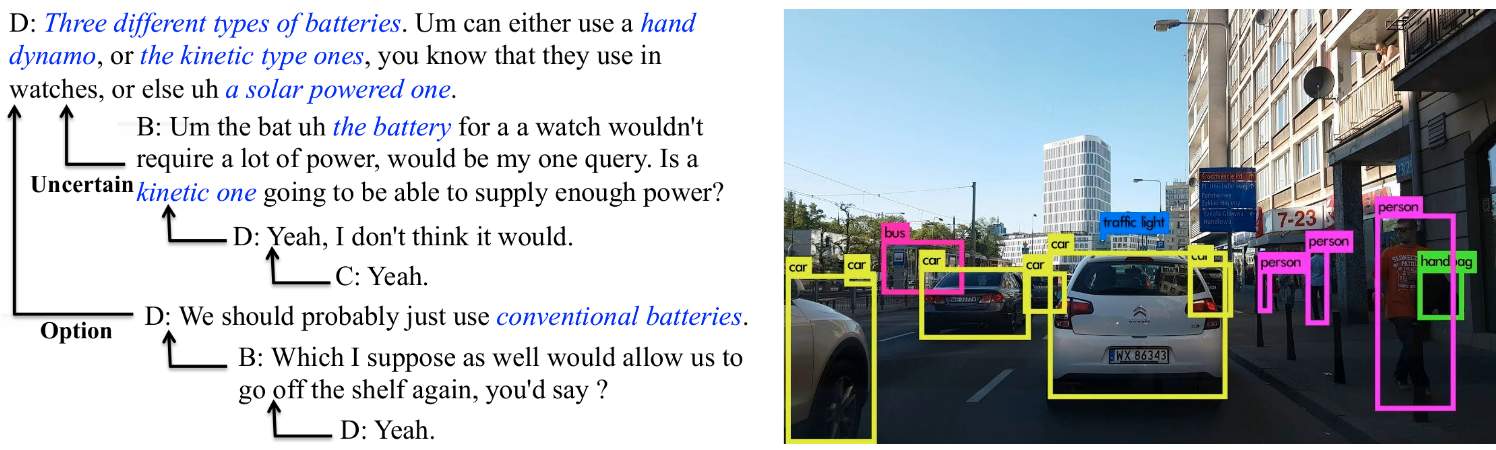
\includegraphics[width=1.0\columnwidth]{Images/intro_txt_car2.png} 
  \caption{\textbf{Left side:} A meeting snippet labeled with key discussion points (in blue) and discussion flow. Discussion flow, which is the latent information behind the text shows the structure of the discussion and the relation between two utterances. It helps with the identification of key discussion points. \textbf{Right side:} A sample image for object recognition task. We highlight bounding boxes and the label of each object. The bounding boxes are latent information and used to help identify objects.}
\end{figure}\label{fig:intro_car} 


Specifically, to capture a hidden state $z$, a mapping from input $x$ to learning target $y$ can be decomposed into two mappings: $z=f_1(x)$ and $y=f_2(z)$. Rather than modeling the distribution $p(y|x)$ directly, we can introduce an unobserved hidden variable $z$ to represent the intermediate state, and define two conditional distributions $p(z|x)$ and $p(y|z)$ for the data. The joint distribution over the target and hidden variable conditioned on the observed input can be written down as:

\[p(y,z|x) = p(y|z)p(z|x)\]

Usually, we can assume that $z$ is a discrete variable. By marginalizing out all possible state of $z$, we obtain the desired data distribution $p(y|x)$:

\[p(y|x) = \sum_z p(y|z)p(z|x)\] \label{eq2}

Model with hidden variables are known as latent variable models (LVM). Latent variable model is proposed to examine latent dependency structure among observable variables. The simplest form of LVM is when $z\in{1,...,K}$, representing a discrete latent state. We will use a discrete prior for this, $p(z_i)=Cat(\pi)$. For the likelihood, we use $p(x_i|z_i=k)=p_k(x_i)$, where $p_k$ is the k'th base distribution for the observations; this can be of any type \cite{murphy2012machine}. The overall model is known as a mixture model. The most widely used mixture model is the mixture Gaussians, also called a Gaussian mixture model (GMM). GMM is one of the most early works in introducing latent variables into machine learning models. Thereafter, latent variable modelling has gradually become an integral part of machine learning research. In text analysis, Probabilistic Latent Semantic Analysis (PLSA) \cite{hofmann2013probabilistic2} and Latent Dirichlet Allocation (LDA) \cite{blei2003latent} are two well-known topic modeling approaches, and both model the topic as a latent variable. In image analysis, it is natural to use latent variables to model human body parts or parts of objects in detection tasks. The work in \cite{wang2006hidden} introduces Hidden Conditional Random Fields, a discriminative probabilistic latent variable model for structured prediction, with applications to two computer vision tasks. In additional to these early LVM works, the combination of latent variable and neural networks has been widely studied in recent years. Chung \cite{chung2015recurrent} propose to integrate recurrent neural networks with latent random variables to model the kind of variability observed in highly structured sequential data. Ji \cite{ji2016latent2} presents a latent variable recurrent neural network architecture for jointly building a language model and understanding latent text information. Gulrajani \cite{gulrajani2016pixelvae2} introduced a VAE model for natural images to learn compressed representations in its latent variables by ignoring the small-scale structure in images. Inspired by all above work, in our thesis we study the usage of LVM with both traditional machine learning models and neural networks.

% LVM and deep learning...

% 2. learning :
% As latent variable models become more and more popular in machine learning community, different learning and inference methods are proposed to estimate model parameters...

For a better story structure, we divide the work into two parts based on two different types of latent information: \textit{sequential data} and \textit{discourse structure}. In chapter \ref{ch-2}, we will first introduce how to model sequential data as latent information in multi-label classification and knowledge based question answering. We analyze existing models proposed for these tasks, and show that existing training and prediction objectives are not well justified mathematically and have undesired consequences in practice. To avoid the drawbacks of existing ones, we develop efficient training and prediction methods by considering latent variables. We also crawl new datasets for multi-label prediction task, and release them for public research. Our experimental results show that our method outperforms state-of-the-art methods. In chapter \ref{ch-3}, we then study in natural language processing (NLP) how discourse structure contributes to understanding human language. Acquiring labeled discourse structures is a time-consuming process since it would require human annotators to inspect the full discourse. Therefore, we propose to model discourse structure as latent variable and jointly infer it with the learning target. In this way, we can solve the task without using additional annotations. Our models show good performances on two standard NLP tasks, text summarization and text based question answering. To further evaluate the correctness of generated discourse structures, we employ human identification and downstream tasks to interpret the output of our models.